%----------------------------------------------------------------------------------------
%	PACKAGES AND OTHER DOCUMENT CONFIGURATIONS
%----------------------------------------------------------------------------------------

\documentclass[11pt, notitlepage]{article} % Default font size and suppress title page

\usepackage[utf8]{inputenc} % Required for inputting international characters
\usepackage[T1]{fontenc} % Output font encoding for international characters
% A note on fonts: As of 2019, NIH allows Arial, Georgia, Helvetica, and Palatino Linotype. Georgia and Arial are commercial fonts so you will need to use XeLaTeX and have them installed on your machine to use them. Palatino & Helvetica are available as free LaTeX packages so select the one you want and comment out the other.
\usepackage{palatino} % Palatino font
\linespread{1.05} % A little extra line spread is better for the Palatino font
%\usepackage{helvet} % Helvetica font
\renewcommand*\familydefault{\sfdefault} % Use the sans serif version of the font

\usepackage{subfig}
\usepackage{listings}
\usepackage{mathtools}
\usepackage{natbib}
\usepackage{color}
\usepackage[normalem]{ulem}
%\usepackage{subcaption}
\usepackage{leading}

\usepackage{amsfonts, amsmath, amsthm, amssymb} % For math fonts, symbols and environments
\usepackage{graphicx} % Required for including images
\usepackage{booktabs} % Nice rules in tables
\usepackage{wrapfig} % Required for text to wrap around figures and tables
\usepackage[labelfont=bf]{caption} % Make figure numbering in captions bold
\usepackage[top=0.5in,bottom=0.5in,left=0.5in,right=0.5in]{geometry} % Page margins
\pagestyle{empty} % Suppress headers and footers

\hyphenation{ionto-pho-re-tic iso-tro-pic fortran} % Specifies custom hyphenation points for words or words that shouldn't be hyphenated at all

%Mathematische Formelabkürzungen%Mathematische Formelabkürzungen
 \newcommand\dd{{\mbox{d}}}
 \newcommand\p{{\partial}}
 \newcommand\beq{\begin{eqnarray}}
 \newcommand\eeq{\end{eqnarray}}
 \newcommand\beqn{\begin{eqnarray*}}
 \newcommand\eeqn{\end{eqnarray*}}
 \newcommand\spa{\vspace{2\baselineskip}\noindent}
 \newcommand\sap{\vspace{\baselineskip}\noindent}
\newcommand{\ab}{\vskip 1cm}
\newcommand\sd{{\mbox D}}
%
\newcommand{\uu}[1]{\underline{#1}}
\newcommand{\pd}[2]{\frac{\partial #1}{\partial #2}}
\newcommand{\pdd}[2]{\frac{\partial^2 #1}{\partial #2^2}}
\newcommand{\ddd}[2]{\text{d}^#1#2}
\newcommand{\dt}{\text{d}t}
\newcommand{\dr}{\text{d}^3r}
\newcommand{\dv}{\text{d}^3v}
\newcommand{\dmu}{\text{d}^6\mu}
%%Mathematische Kuerzel
%\def\mund{{\hspace{0.5cm} \rm und} \hspace{0.5cm}}
%\def\mfalls{{\hspace{0.5cm} \rm falls} \hspace{0.5cm}}
%\def\mmit{{\hspace{0.5cm} \rm mit} \hspace{0.5cm}}
%\def\mor{{\hspace{0.5cm} \rm or} \hspace{0.5cm}}
%\def\mpunkt{{\hspace{0.5cm} \rm .}}
%\def\mkomma{{\hspace{0.5cm} \rm ,} \hspace{0.5cm}}
%\def\many{{\hspace{0.5cm} \rm any} \hspace{0.5cm}}
%\def\hasp{\hspace{0.5cm}
%\def\mconst{{\rm const.}}
%%Aufteilung
%\setcounter{topnumber}{10}
%\setcounter{bottomnumber}{10}
%\setcounter{totalnumber}{10}

%Heikki's definitions, from original NumericalExp.tex
\newcommand{\vdag}{(v)^\dagger}
\newcommand{\md}[1]{\frac{D #1}{D t}}
\newcommand{\td}[2]{\frac{\rm d #1}{\rm d #2}}
\newcommand{\vn}{\vec \nabla}
\newcommand{\pdgs}[2]{\frac{\partial #1}{\partial #2}{\Big |}_o}
\newcommand{\tsub}[2]{#1_{\mbox{\tiny #2}}}

\def\ppder{\mathaccent "7F }
\def\pder{\mathaccent 95 }
\def\vdisp{\sqrt{<v^2>}}
\def\pr{\mathaccent "7F }

\newcommand{\Fvec}{\vec F}
\newcommand{\rppvec}{\ppder{\vec r}}
\newcommand{\rpvec}{\pder{\vec r}}
\newcommand{\rvec}{\vec r}
\newcommand{\vvec}{\vec v}
\newcommand{\dvvec}{\Delta \vec v}
\newcommand{\drvec}{\Delta \vec r}
\newcommand{\drpvec}{\Delta \pder{\vec r}}
\newcommand{\pvvec}{\vec {\mathaccent 95 v}}
\newcommand{\pgvec}{\vec {\mathaccent 95 g}}
\newcommand{\pkvec}{\vec {\mathaccent 95 k}}

\newcommand{\qvec}[1]{R_{#1} \vec \omega_{#1}}
\newcommand{\ovec}{\vec \omega}
\newcommand{\Ovec}{\vec \Omega}

\newcommand{\kvec}{\vec k}
\newcommand{\ktvec}{{\vec k}_T}
\newcommand{\kgvec}{{\vec k}_\gamma}

\newcommand{\gvec}{\vec g}
\newcommand{\dgvec}{\Delta \vec g}
\newcommand{\gpost}{{\vec g}^\prime}

\newcommand{\qa}{\vec q}
\newcommand{\qb}{\vec q_1}
\newcommand{\qs}{\vec q_s}

\newcommand{\dqa}{\Delta \vec q}
\newcommand{\dqb}{\Delta \vec q_1}
\newcommand{\dqs}{\Delta \vec q_s}


\newcommand{\ma}{m\alpha}
\newcommand{\mb}{m_1\alpha_1}

\newcommand{\en}{\epsilon_N}
\newcommand{\et}{\epsilon_T}
\newcommand{\eg}{\epsilon_\gamma}

\newcommand{\meff}{m_{\rm eff}}

\newcommand{\ff}{f\hspace{-4pt}f}

%Thomas Orgis <thorgis@rz.uni-potsdam.de>
\newcommand \ham {{\hat{\bf H}}}
\newcommand \stat {\ket{{\cal S}}}
\newcommand \ew[1] {\langle #1 \rangle}
\newcommand \gew[1] {\left\langle #1 \right\rangle}
\newcommand \ket[1] {\vert #1 \rangle}
\newcommand \bra[1] {\langle #1 \vert}
\newcommand \braket[2] {\langle #1 \vert #2 \rangle}
\newcommand \brakett[3] {\langle #1 \vert #2 \vert #3 \rangle}
\newcommand \vecop[1]  {\hat{\vec {\bf #1}}}
\newcommand \op[1] {\hat{{\bf #1}} }
%\newcommand \prodnotiz[1] {\begin{center}\fbox{\begin{minipage}{\textwidth}--- TIPPER-KOMMENTAR: #1 ---\end{minipage}}\end{center}}
\newcommand{\R}{\mathbb{R}}
\newcommand \gkl[1]{\left( #1 \right)}
\newcommand \egk[1]{\left[ #1 \right]}
\newcommand \ggk[1]{\left\{ #1 \right\}}
\newcommand \pdt {\frac {\partial}{\partial t}}
\newcommand \ddt {\frac {\text d}{\text dt}}
\newcommand \dede[2] {\frac {\text d#1}{\text d#2}}
\newcommand \dtt[1] {\frac {\text d^2}{\text d##^2}}
\newcommand \rand[1] {\left. {#1} \right|}
%totales Differatial bei 2 Variablen
\newcommand \totdif[3] {\rand{\pd {#1}{#2}}_{#3} \text d #2 + \rand{\pd {#1}{#3}}_{#2} \text d #3}
%Schwarz-Partielles-Differential
\newcommand \spd[3] {\frac {\partial^2 #1}{\partial #2 \partial #3}}
\newcommand \Rar \Rightarrow
\newcommand \Lar \Leftwarrow
\newcommand \Lrar \Leftrightarrow
\newcommand \rar \rightarrow
\newcommand \lar \leftwarrow
\newcommand \lrar \leftrightarrow
\newcommand \abs[1] {\left | ## \right |}
\newcommand \grad {\text{grad}}
\newcommand \rot {\text{rot}}
\newcommand \di {\text{div}} 

%----------------------------------------------------------------------------------------

\begin{document}

%----------------------------------------------------------------------------------------
%	GENERAL INFORMATION
%----------------------------------------------------------------------------------------

\begin{center}
{\Large \textbf{Project Description:}}\\  
\vspace{.5cm}
{\LARGE\textbf{Project Name}} 
\\[.75cm] 
submitted by\\
{Yernur Baibolatov\\
Universit\"at Potsdam\\
Institut f\"ur Physik und Astronomie}
\end{center}
%\\[.75cm] 
\noindent\textbf{Specific academic field (specialization)}:  Theoretical Physics/Space Science
\\[.75cm] 
\textbf{Supervisor and first expert reviewer for recommendation letters}: \,  Prof. Dr. Frank Spahn
\\[.75cm] 
\textbf{Further expert reviewers (name, academic field; these do not have to be identical with the second reviewer of the PhD thesis)}: \, Prof. Dr. J\"urgen Schmidt \,
\\[.75cm] 
\textbf{Working environment}: ~ The planned studies  will be carried place in the \emph{theoretical planetology} group of Prof. Dr. Frank Spahn of the  \emph{Dpt. 
of theoretical physics}, chair Prof. Dr. Ralf Metzler, where room, working place/space and computer environment will be provided (see signed affirmation attached).

%Please  briefly  explain  how you  are  integrated  in  colloquia, a  working  group,   a  research  training group etc.  Please indicate if you are an individual doctoral student.
\newpage
\section*{Abstract}

Our work concerning cosmic granular gases (planetary rings) has been greatly inspired by the stunning results of the unique  
\emph{Cassini}-mission to the giant-planet Saturn\footnote{Frank Spahn is a member (CoI) of the \emph{Cassini}-CDA (cosmic dust analyzer)
\emph{Science} team since 1995.}. The occultation- (UVIS) and the imaging (ISS) experiments have spotted quite unexpected 
\emph{fine-scale} structures during the \emph{grande finale} phase of that gorgeous mission -- 
clustering structures which occur on the scale of the ring-aggregate sizes as an expression 
of the non-equilibrium character of the huge granular gas disks.\\

We plan to explain these observations with generalized kinetic Boltzmann-type equations addressing aggregation, fragmentation and 
restitution \citep{spahn2004} as collisional results. The latter are quantified by visco-elastic adhering collision dynamics of 
granular icy aggregates \citep{brilliantov2007a}.

In a first step, the evolution of a homogeneous, unperturbed ring composed of aggregates with different masses ($k$ index) is 
analyzed with the zeroth'- and second order mean field-equations, i.e.  the particle number density $n_k (\vec r, t)$ and 
corresponding granular temperatures $T_k (\vec r, t)$. For a given size(mass) distribution (DF) ~ $n_k  \propto k^{-\alpha}$, 
we have found mass ($k$) dependent temperatures $T_k $ as a stationary expression for the non-equilibrium character of the sheared 
granular gas a planetary ring is made of.

In order to investigate cluster formation under external excitations, the \emph{stability} of the steady state solutions will 
be analyzed against gravitational (resonant) perturbations, i.e. we will aim at responses of the size distribution $n_k$ vs 
granular temperatures $T_k$ under external driving.
  
Furthermore, the generalized kinetic model allows to study the momentum and energy transports between different mass 
classes of aggregates relevant for cluster processes and the establishment of vertical stratification.  The different mobilities 
corresponding to ring aggregates of different masses may cause size(mass) segregation processes in a perturbed multi-disperse 
ring. This may lead to a separation of regions containing larger aggregates from those composed of rather small grains -- effects 
which are potentially suitable to describe small scale structural phenomena discovered by \emph{Cassini}.\\
 
 
 \begin{figure}[ht]
	\centerline{
	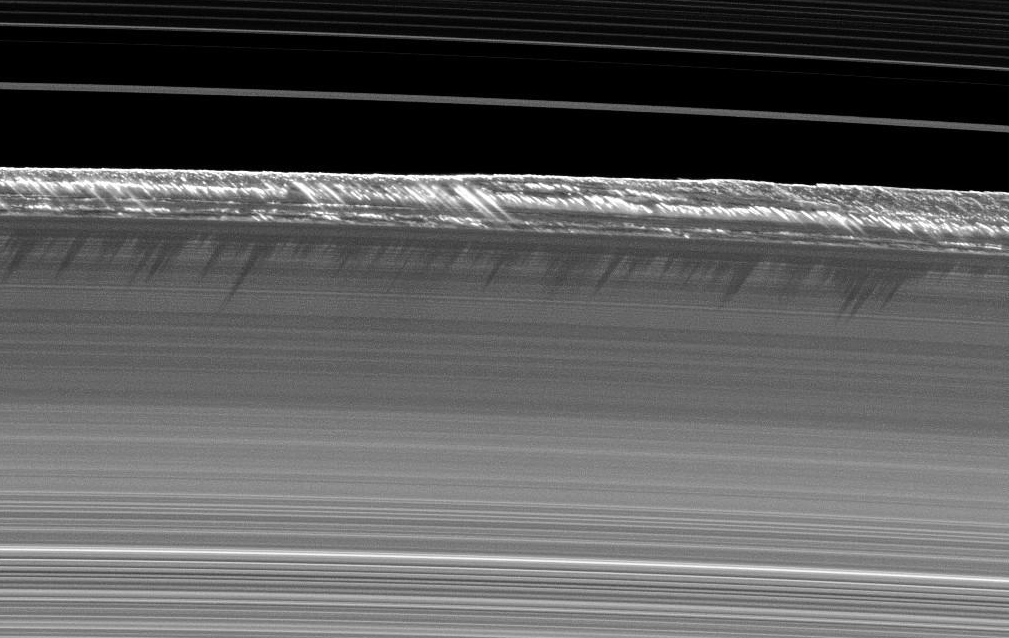
\includegraphics[width=.7\textwidth]{Figures/B_Ring_Edge.png}
	}
	\caption{\small%
%
This Cassini-image taken in August 2009 (Saturn's equinox) shows the outer edge (bright fuzzy horizontal region in the upper 
half of the picture) of  Saturn's dense B ring. The direction from the bottom to the top points radially away from Saturn.  This edge 
-- confined by the 2:1 mean motion resonance of the moon Mimas, the strongest inner resonance acting in the main rings of 
Saturn --  is dominated by inclined, sheared bright features. They cast long shadows onto the ring plane indicating a stunning 
vertical extent of a few kilometers of these remarkable features (Image credit: NASA-JPL).
%
}
\label{B_edge_Alpen}
\end{figure}
 
 %Then our results will be related to those of an empirical low dimensional (2D) kinetic model invented by \citet{esposito2012}, which 
 %are suitable to explain the \emph{Cassini}-observations of the (dynamically changing) shadows and clusters at the outer edge of the B ring of 
% Saturn fairly well.
    
    %We will also apply our modeling to explain triggered clustering in the numerous perturbed regions observed by the Cassini mission, e.g. between density wave crests, caused by resonant interactions, where low granular temperatures promote cluster formation. These theoretical studies will be complemented by a systematic inspection of Imaging- and occultation data gathered by Cassini.


%----------------------------------------------------------------------------------------
%	Summary of the research topic
%----------------------------------------------------------------------------------------

\newpage

\section*{A. Summary of the research topic}

\subsection*{Introduction \& State of ``the Art''}

Saturns rings do not only fascinate the observer by their miraculous beauty, but they are also natural 
``laboratories'' or even proxies for the dynamics of all the cosmic disks of quite different size and distance from us.
These larger ``brothers'' of planetary rings -- e.g. pre-planetary gas-dust disks as the ``nurseries'' of planets,
the huge galactic disks or spirals -- have many physical processes in common with dense planetary rings as
for instance:  differential rotation or quite a low ratio between vertical and lateral extent. The advantage of
those cosmic disks in our cosmic neighborhood is that we can inspect these objects in situ with space-vehicles.\\


During its 13 years-journey through the Saturnian system, the \emph{Cassini}-spacecraft has detected a wealth of new
structures and phenomena in Saturn's dense, icy granular rings. For instance, there have been a confirmation
of  ``viscous overstabilities'' \citep{thomson2007} or ``propeller'' structures caused by ``skyscraper''-sized tiny
ring-moons (dubbed as moonlets; \citeauthor{tiscareno2006}, \citeyear{tiscareno2006}) -- both formerly theoretically predicted
in our group \citep{schmidt2001,spahn2000b}.\\
Density- and bending waves -- driven by the gravity action of the numerous Kronian satellites or structural inhomogeneities 
inside Saturn and first spotted by the \emph{Voyager}-cameras -- have now been caught with the camera-system (Imaging Sub-System -
ISS) of the \emph{Cassini}-spacecraft  at an unprecedented spatial resolution \citep{French2016,Tiscareno2018}. These spiral waves are 
dominated by inertia forces -- acting in a differentially rotating  Keplerian ring --  balanced by the self-gravity of the ring-matter providing a 
possibility to estimate the local mass density of the ring.
\begin{figure}[ht]
	\centerline{
	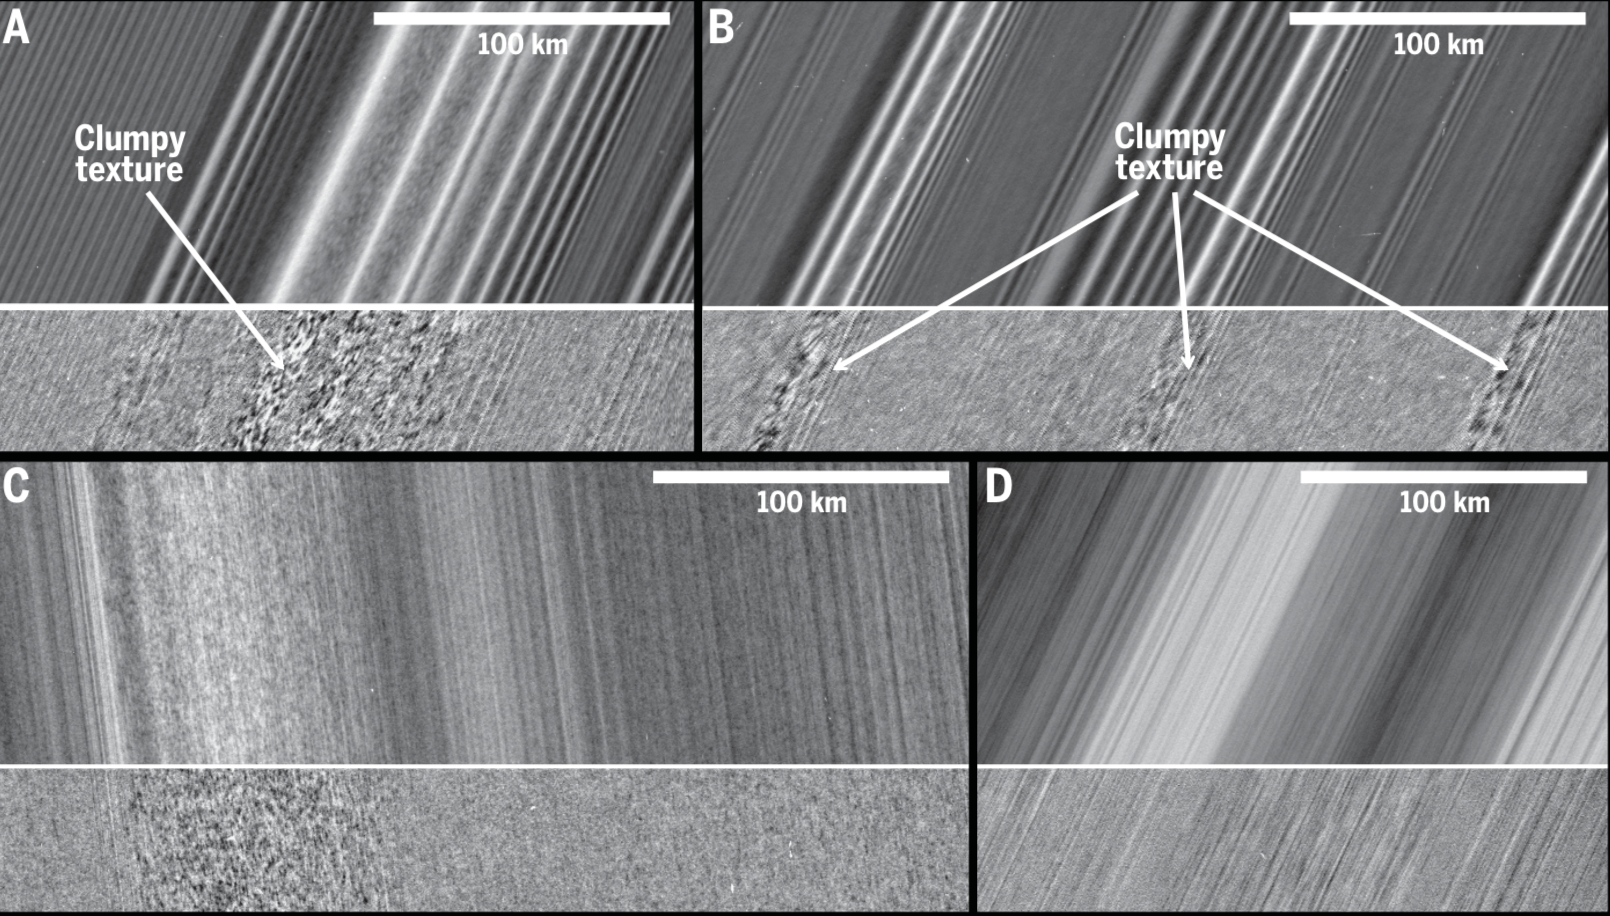
\includegraphics[width=.7\textwidth]{Figures/Strawing.png}
	}
	\caption{\small
In resonantly driven density waves in Saturn's rings (upper panels A \& B) a clustering texture mainly appears in the wave troughs, 
characterized by low granular temperatures usually corresponding to larger mean sizes \citep{goldhirsch1993,esposito2012}  
(Image from \citet{Tiscareno2019}).
}
\label{WavesStraw}
\end{figure}
Apart from those already expected ring-phenomena, new features have been caught by \emph{Cassini's} cameras (ISS-data) as 
presented in Figure \ref{B_edge_Alpen}. Here the B ring edge --  confined by the strongest 
resonance in the rings: the 2:1 inner Mimas Lindblad resonance -- is shown with its tilted \emph{fine-structures} 
in the grazing Sun-light during the sunset at the rings (equinox in August 2009). Under these illumination conditions all outstanding 
vertical features cast shadows whose lengths provide a measure for the vertical extent of these structures. Those visible in 
Figure \ref{B_edge_Alpen} suggest a 3.5 kilometre  altitude of vertical ring-matter excursions \citep{spitale2010}. Having a closer 
look at this image, it seems that the shadows are closely tied to the inclined bright streaky features/clusters suggesting their quite large 
vertical reach.

Further examples of unexpected material clustering are shown in Figure \ref{WavesStraw} which occur in regions of resonantly driven 
waves in Saturns rings. 

All these observations indicate that larger clusters preferably evolve in ``colder'', unperturbed regions where the collision frequency and
-intensity is reduced. \citet{esposito2012} have described these facts with a two-dimensional, scale-based kinetic model quantifying
evolution of two state variables: \, the  \emph{mean effective mass} $\approx \ew{k}$ along with the \emph{mean velocity dispersion} 
$\approx \ew{T_k}$  (mean granular temperature), which covers astonishingly well the \emph{Cassini}-observations\footnote{The mass-index
$k$ labels the number of constituents forming a ring-aggregate of mass $m = k m_0$}.

Based on a generalized kinetic theory \citep{spahn2004,spahn2014} we have calculated the size-spectrum $n_k$ under near-equilibrium
conditions \citep{Brilliantov2015}, i.e.  assuming energy equipartition of all mass-classes $T_k \rightarrow T$. The result is shown 
in Figure \ref{SizesDF} attesting an astonishingly well agreement with spacecraft measurements. 
\begin{figure}[ht]
	\centerline{
	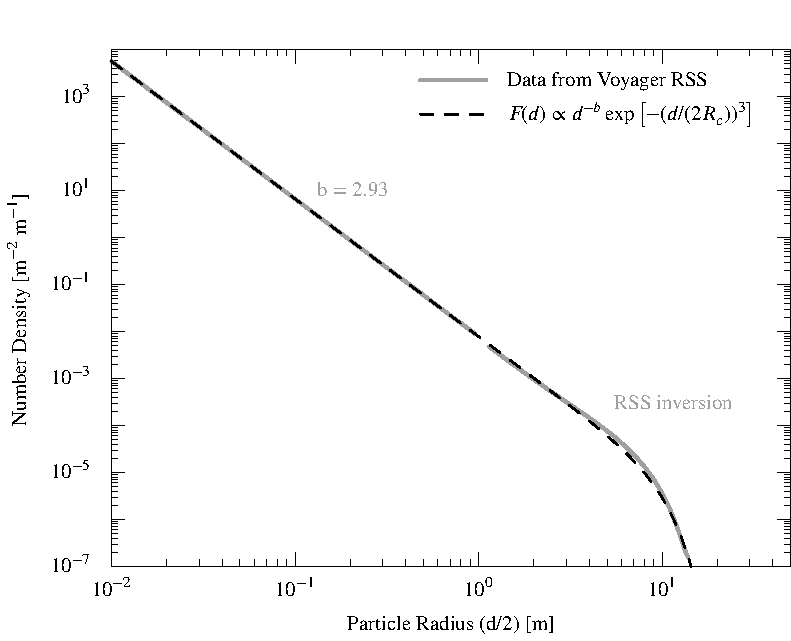
\includegraphics[width=.5\textwidth]{Figures/sdfa219b}
	}
	\caption{\small
The particle size distribution obtained by \citet{Brilliantov2015} compared to the Voyager radio-science (RSS) data.
A quite good agreement between theory and observation has been found.}
\label{SizesDF}
\end{figure}
\sap

However, even these obvious successes of the above models do not hide the fact that neither a two-dimensional
reduction \citep{esposito2012} nor the assumption energy-equipartition \citep{spahn2004,Brilliantov2015} are sufficient
to explain the non-equilibrium character of the fine-scale structures observed in Saturn's rings. Consequently, we
have started to investigate the coupled dynamics of the granular temperatures $\ggk{T_k}$ with the 
mass-frequencies $\ggk{n_k}$ of an undisturbed dense ring\footnote{The curly brackets denote the ${\cal N}$-tuples
of the mass-classes.}. A splitting up of an universal temperature into a mass-dependent spectrum $T \rightarrow \ggk{T_k}$
has been found as an expression of the non-equilibrium character of the undisturbed multi-disperse sheared granular gas!

In the planned project, we will analyze the stability of that steady state under external perturbations in order to understand the
cluster formation, and thus, to complete the goals of my PhD-thesis!\\

\subsection*{Scientific Objectives}
Unlike molecular gases, a granular gas is always subject to collisional dissipation of inner 
energy, hence temperature decay over time \citep{Haff1983, Brilliantov2004}. Even more interesting phenomena can be
observed when granular gas consists of species with different masses. In this case, 
due to non-equal partitioning of energy, each species attain unique granular
temperatures \citep{Garzo2007c, Osinsky2020}. 

The model we consider is a granular gas with polydisperse size-distribution 
of constituents in a sheared environment. We start our kinetic description of such a medium 
with an introduction of a one-particle DFs $f_k(\vec{r}, \vec{v}, t)$ for each species $k$. Time evolution of such functions 
obey Boltzmann-type kinetic equations \citep{Haff1983, Brilliantov2004}:
\begin{equation}\label{eq:kinetic}
	\frac{\partial f_k}{\partial t}+\vec{v}\cdot\frac{\partial f_k}{\partial\vec{r}}-
	\frac{1}{m_k}\frac{\partial U}{\partial\vec{r}}\cdot\frac{\partial f_k}{\partial\vec{v}}=
	\sum_i n_iI_c(f_k,f_i)\;,
\end{equation}
where $U(r)$ is the gravitational potential of the planet and $I_c(f_k, f_i)$ is the collision integral. Using these DFs we 
can introduce macroscopic fields as corresponding velocity moments of DFs:
\begin{equation}
	\begin{split}
		\rho_k(\vec{r}, t) &= m_k\int f_k(\vec{r}, \vec{v}, t)\,d\vec{v}\;,\\
		\rho_k(\vec{r}, t)\vec{u}(\vec{r}, t) &= \int \vec{v}f_k(\vec{r}, \vec{v}, t)\,d\vec{v}\;,\\
		T_k(\vec{r}, t) &= \frac{2}{3}\int \frac{m_k c^2}{2}f_k(\vec{r}, \vec{v}, t)\,d\vec{v}\;,
	\end{split}
\end{equation}
where $\rho_k=m_kn_k$ is the mass density, $\vec{u}$ is the mean velocity and $\vec{c}=\vec{v}-\vec{u}$ is the peculiar velocity.
Multiplying Eq.~(\ref{eq:kinetic}) by necessary power of velocity and integrating over the whole velocity space, we obtain 
corresponding mean field balance equations. In a generic form, for any given macroscopic field $F_k(\vec{r},t)$, these balance equations 
are in the next form:
\begin{equation}
	\left\langle\frac{dF_k}{dt}\right\rangle_{convective}=\left\langle\frac{dF_k}{dt}\right\rangle_{collisional}\;,
\end{equation}
meaning that convective changes of the field are balanced by the collisional changes. In our first step, we consider only restitutive 
collisions, meaning that size-distribution function does not change. In this case, due to mass and momentum conservation, the 
zeroth and first order moment equations have no collisional changes. The second moment equations, i.e. temperature evolution equations,
give us much more interesting information, since they have non-zero collisional changes. In a generalized form, these equations can be written as:
\begin{equation}
	\frac{dT_k}{dt} \propto H_k -A_kT_k+\sum_{i}B_{ki}(T_k-T_i)\;,
\end{equation}
where $A_k>0$ is the parameter describing 
dissipation due to collisions, which depends on size distribution function, collision 
frequency and restitution. The parameter $B_{ki}=B_{ik}>0$ describes the inter-species 
heat flow. This is the main reason why species tend to have different temperatures. 
$H_k$ is a certain external heating function. If one introduces an external energy pump 
into the system, the temperatures of species don't reach zero, but attain certain 
stationary and still unique values, balancing the outer heating \cite{Bodrova2014}. 

One caveat of these heating models is that they are all artificial. Our goal 
is to investigate the model with a more realistic heating term, the gravitational 
shear heating in planetary disks. This heating is in the next form:
\begin{equation}
	H_k \propto \nu_k\Omega^2\;,
\end{equation}
where $\Omega$ is the mean orbital frequency around the considered location of the system,
and $\nu_k$ is the shear viscosity term. In the case of planetary rings, the viscosity
term is split into \emph{local} and \emph{non-local} parts $\nu=\nu_l+\nu_{nl}$ 
\cite{Seiss2011,spahn2006c,Stewart1984}.
However, these terms are given only for the mono-disperse case. In the case of a gas 
with different species, we need to know the viscosity terms for each species. 
This is the first goal of our project, to obtain the kinetic transport coefficients
for each species from the microscopic level of description. 
By this we mean kinetic description of the system, given a velocity distribution 
function $f$, its time evolution obeys:

In order to test the theoretical results, we have developed a molecular dynamics (MD) 
code, simulating granular particles of different sizes in a Hill's box. 
\emph{Here some $\ln T$ over $\ln t$ simulation results graph Fig.~\ref{fig2}}
\begin{figure}[h] % Figure at bottom of the page ([b] argument, could be "t" for top or "h" for here)
	\centering
	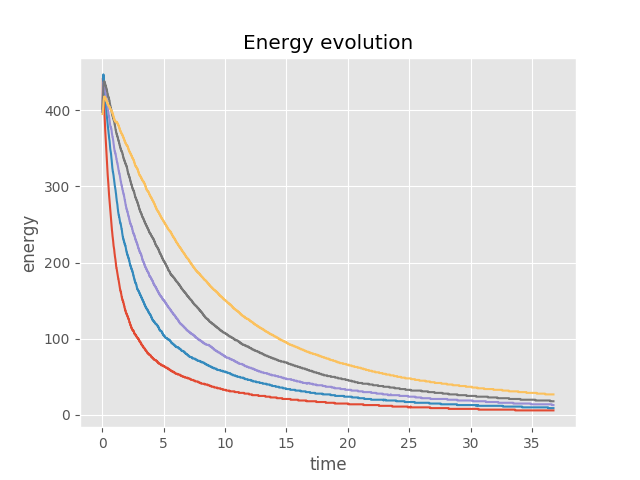
\includegraphics[scale = .80]{Figures/energy_evo.png}
	\caption{\footnotesize This is only an example plot. Should be replaced by my new simulation results}
	\label{fig2}
\end{figure}

Next, we would like to address the reasons for size distribution in Saturn's rings. 
From experimental evidence, we that the size distribution obeys a power
law with a cut-off at the end [size-distribution tail original works]. There are several attempts
to model this phenomenon \cite{Brilliantov2013,spahn2014}. All of them assume a certain interplay between
two driving processes, aggregation or coagulation process when particles merge, producing 
larger particles, and fragmentation process, when particles
fracture after collision producing smaller constituents. A natural step for us would be 
to analyze the kinetic equations describing the behavior of the system with inclusion 
of aggregation and fragmentation processes.

Such an interplay and balance of three different processes, one being separation of 
temperatures of species, second being the gravitational heating and third 
being the recombination of particles which lead to dynamical change of size distribution,
is already quite interesting. Hence, an external influence, such as periodic 
driving force acting upon the system should lead to various fascinating phenomena.
In planetary systems, such periodic driving forces are resonances with the moons of the 
planet.

%----------------------------------------------------------------------------------------
%	Table of contents and outline of the thesis with an overview of accomplished (sub-) chapter
%----------------------------------------------------------------------------------------

\spa
\section*{B.Table of contents and outline of the thesis with an overview of accomplished (sub-) chapter}
Please submit your table of contents /outline of your thesis. Please characterize the (sub-)chapter 
that have already been accomplished. 
The probability of concluding the project during the funding period must be illustrated. 
The awarding committee reserves the right to obtain the stated (sub-) chapter in printed form.

%----------------------------------------------------------------------------------------
%	Working program and intended completion date
%----------------------------------------------------------------------------------------

\newpage
\section*{C. Working program and intended completion date}
\begin{itemize}
    \item Working-Program, time schedule (max. 4 pages)Detailed information about your planned approach, especially a thorough explanation of the meth-odology, 
	that you will apply in the completion phase of your  PhD. A time schedule (e. g. in graphic or  tabular  form)  for  the  period  of  
	funding  should  clearly  demonstrate  the  steps  in  your  research  project that are planned, have already started or are completed. 
	If your PhD includes experiments, please indicate the experiments that have already been conducted and that will still be conducted. 
	The  quality  of  the  research  approach  and  the  characterization  of  the  accomplished  and  planned  steps are of utmost importance.
    \item Please specify your intended completion date.
\end{itemize}
%----------------------------------------------------------------------------------------
%	Literature
%----------------------------------------------------------------------------------------

\newpage
\section*{D. Literature}

%\newpage

{\small
\bibliographystyle{apalike}
%\renewcommand\bibsection{\section{\refname}}
%\renewcommand{\refname}{Bibliography}
%\bibliography{project}
\bibliography{Mergedbib,Pape} % Use the NIHGrant.bib file for the reference list, replace with your own
%\bibliographystyle{nihunsrt} % Use the custom nihunsrt bibliography style included with the template
}

%----------------------------------------------------------------------------------------

\end{document}